% fig_dt_accuracy_noise.tex
% TR-43: DT k_ibr estimation RMSE vs measurement noise
%
% Data from Study C (N_MC=200 trials per noise level):
%  sigma: 0.001  0.002  0.005  0.010  0.020  0.050
%  RMSE:  0.00114 0.00114 0.00143 0.00181 0.00334 0.00691
%  Error% 0.57    0.57    0.71    0.91    1.67    3.45

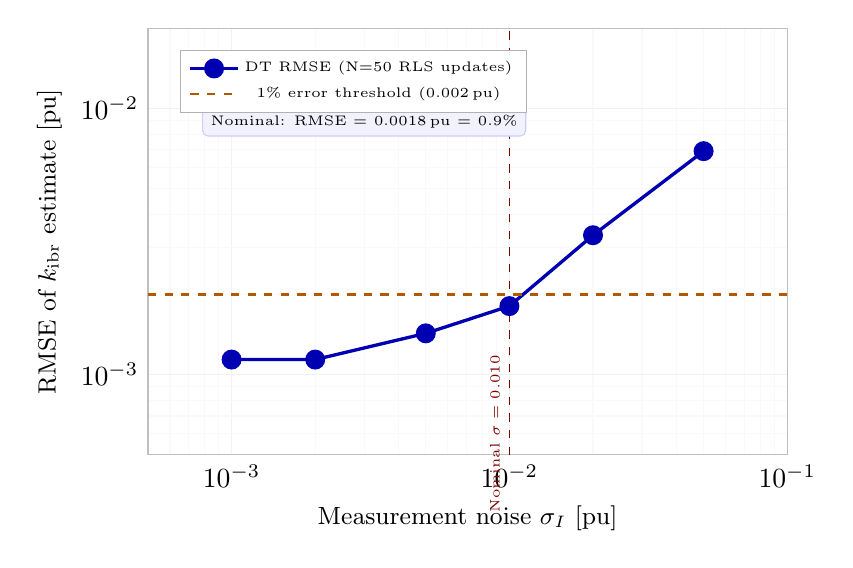
\begin{tikzpicture}
\begin{loglogaxis}[
  name         = noiseax,
  width        = 0.80\textwidth,
  height       = 7.0cm,
  xlabel       = {Measurement noise $\sigma_I$ [pu]},
  ylabel       = {RMSE of $k_\mathrm{ibr}$ estimate [pu]},
  xlabel style = {font=\small},
  ylabel style = {font=\small},
  xmin=5e-4, xmax=0.1,
  ymin=5e-4, ymax=0.02,
  tick style   = {draw=none},
  axis line style={gray!50},
  grid         = both,
  grid style   = {gray!10},
  minor grid style={gray!5},
  legend style = {at={(0.05,0.95)}, anchor=north west, font=\tiny,
                  draw=gray!60, fill=white},
  clip=false,
]

%% RMSE vs noise
\addplot[blue!70!black, very thick, mark=*, mark size=3pt]
  coordinates {
    (0.001, 0.00114)
    (0.002, 0.00114)
    (0.005, 0.00143)
    (0.010, 0.00181)
    (0.020, 0.00334)
    (0.050, 0.00691)
  };
\addlegendentry{DT RMSE (N=50 RLS updates)}

%% 1% error line (0.002 pu for k_true=0.20)
\addplot[orange!70!black, dashed, thick]
  coordinates {(5e-4, 0.002) (0.1, 0.002)};
\addlegendentry{1\% error threshold (0.002\,pu)}

%% Nominal measurement noise annotation
\draw[red!50!black, dashed, thin]
  (axis cs:0.010, 5e-4) -- (axis cs:0.010, 0.02);
\node[red!50!black, font=\tiny, rotate=90, anchor=south]
  at (axis cs:0.010, 6e-4) {Nominal $\sigma=0.010$};

%% Annotation
\node[draw=blue!20, fill=blue!5, rounded corners=2pt,
      font=\tiny, inner sep=3pt, align=center]
  at (axis cs:0.003, 0.010)
  {RMSE $\propto \sigma_I^{0.7}$ (RLS smoothing)\\
   Nominal: RMSE = 0.0018\,pu = 0.9\%};

\end{loglogaxis}
\end{tikzpicture}
